\documentclass[12pt]{article}

\usepackage[margin=3cm]{geometry}
\usepackage{amsmath, amssymb, amsthm}
\usepackage{url}
\usepackage{graphicx}
\usepackage{eqlist}
\usepackage{uri}
\urisetup{doipre={https://doi.org/}}
\usepackage{natbib}
\usepackage{siunitx}
\usepackage{pythonhighlight}
\usepackage{comment}
\usepackage{caption}
\usepackage{tabularx}
\usepackage{tikz}
\usepackage{tasks}
\usepackage{oubraces}
\usepackage[inline]{enumitem}
\usepackage{titling}
\usepackage{tcolorbox}
\tcbuselibrary{breakable}
\usepackage{needspace}
\usepackage{fancyhdr}
\usepackage[font={small}, labelfont=bf]{caption}
\captionsetup{width=.7\textwidth, font=small}
\usepackage{hyperref}
\usepackage{forest}
\hypersetup{
    colorlinks=true,
    urlcolor=blue,
    % hidelinks=true,
    linkcolor=black,
    citecolor=black,
}
\usetikzlibrary{positioning} 
% set the float page fraction
\renewcommand{\floatpagefraction}{.8}

% Initialize line spacing to 1.5
\linespread{1.5}

% Define \sgn function
\DeclareMathOperator{\sgn}{sgn}
\DeclareMathOperator{\real}{Re}
\DeclareMathOperator{\imag}{Im}
\DeclareMathOperator{\Ei}{Ei}
\DeclareMathOperator{\E1}{E_1}
\DeclareMathOperator{\atan2}{atan2}
\DeclareMathOperator{\lcm}{lcm}
\DeclareMathOperator{\gcf}{gcf}

% Simple exercises environment using basic enumerate
\newcounter{exercisenum}
\newenvironment{exercises}{%
  \begin{tcolorbox}[colback=white,colframe=black,arc=0pt,breakable]
%   \noindent\textbf{Exercises}\par
  \begin{enumerate}[label=\arabic*),leftmargin=1cm,resume=exercises]
  \setcounter{enumi}{\value{exercisenum}}
}{%
  \setcounter{exercisenum}{\value{enumi}}
  \end{enumerate}
  \end{tcolorbox}
}

% Setup footer for first page only
\fancypagestyle{firstpage}{
  \fancyhf{}
  \fancyfoot[L]{\small FACTORS EXTENSION}
  \fancyfoot[R]{\small \quad Ewan Short \quad \today}
  \fancyfoot[C]{\small\thepage}
  \renewcommand{\headrulewidth}{0pt}
  \renewcommand{\footrulewidth}{0pt}
}

\begin{document}

\thispagestyle{firstpage}

\section{Secret Level (Optional!)}

\begin{itemize}
\item
Let's write the least common multiple of two whole numbers $a$ and $b$ as $\lcm(a,b)$. For example,
$$\lcm(2,3) = 6,\quad\quad \lcm(6, 8) = 24.$$
Note the order doesn't matter here, $\lcm(a,b) = \lcm(b,a)$.
\end{itemize}
\begin{exercises}
\item
The 166 bus arrives at Wyndham Vale Station every 44 minutes, and the 192 bus every 36 minutes. If both buses arrive at 10:00 AM, when do they next arrive together? \textit{Hint}: find $\lcm(44,36)$. \phantom{04:36 PM.}
\item 
Sometimes $\lcm(a,b)=a\times b$, but sometimes not. For example,
\begin{align*}
\lcm(2,3) &= 6 = 2\times 3,\\
\lcm(4,6) &= 12 \ne 4\times 6 = 24.
\end{align*}
Under what circumstances is $\lcm(a,b) = a\times b$?
\end{exercises}

\begin{itemize}
\item
The \underbar{greatest common factor} of two whole numbers is the \underbar{largest} whole number that divides both without remainder. Let $\gcf(a,b)$ denote the greatest common factor of $a$ and $b$. For example,
$$
\gcf(12, 18) = 6,\quad\quad \gcf(4, 8) = 4.
$$
Order doesn't matter here, $\gcf(a,b) = \gcf(b,a)$.
\item
We can find the greatest common factor of two numbers using prime decomposition, just like with the least common multiple. But this time if a factor is in both original numbers and the indices are different, we use the \underbar{smaller} index. For example,
$$
\begin{array}{lll}
12 = 3^1\times 2^2, & 18 = 2^1\times 3^2, &\text{so } \gcf(12,18)=2^1\times 3^1 = 6. \\
4 = 2^2, & 8 = 2^3, &\text{so } \gcf(4, 8)=2^2=4.
\end{array}
$$
\end{itemize}

\begin{exercises}
\item
You're tiling a tiny $\SI{12}{\centi\meter} \times \SI{8}{\centi\meter}$ section of bathroom floor. You have square tiles with sides $\SI{1}{\centi\meter}, \SI{2}{\centi\meter}, \SI{3}{\centi\meter}, \ldots$ What's the largest square tile you can use without cutting them up? \textit{Hint:} Find $\gcf(12, 8)$, then draw the tiles on the grid below to check your answer!
\begin{center}
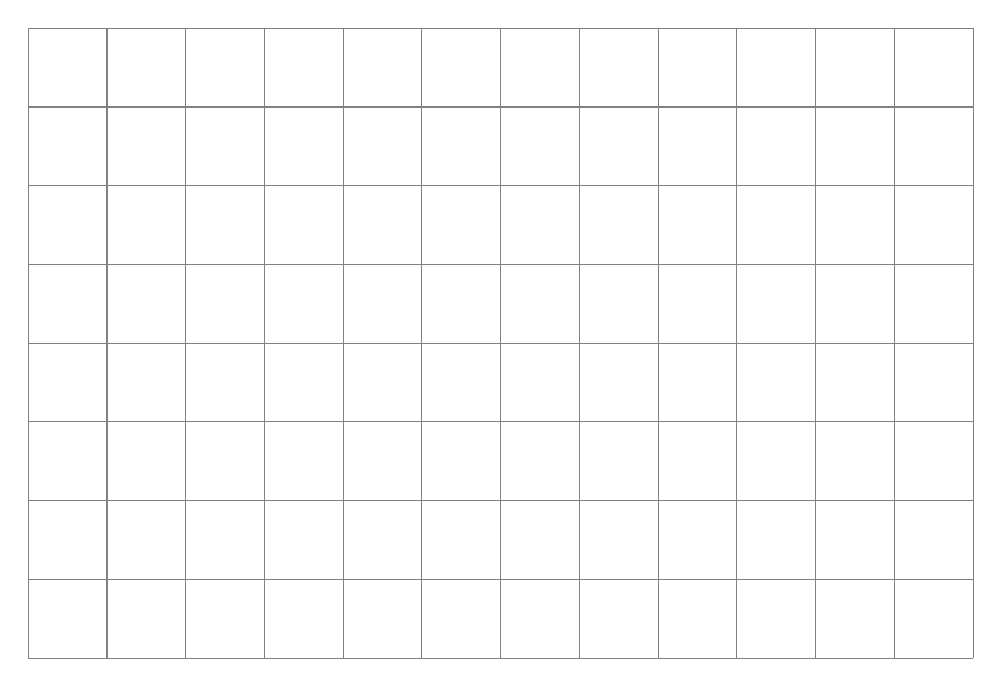
\begin{tikzpicture}
\draw[step=1cm, gray, thin] (0, 0) grid (12, 8);
\end{tikzpicture}
\end{center}
\item
For any positive whole numbers $a$ and $b$,
$$
\lcm(a,b)\times\gcf(a,b) = a\times b.
$$
Test this relationship with $a=12$ and $b=18$. Can you explain why the relationship is always true?
\end{exercises}

\bibliographystyle{ametsocV6}
\bibliography{references}

\end{document}